\documentclass{beamer}

\beamertemplatenavigationsymbolsempty

\usepackage{tikz}

\usetikzlibrary{positioning}
\usetikzlibrary{shapes,arrows,calc}

\definecolor{variable}{HTML}{999999}
\definecolor{operator}{HTML}{bbbbbb}
\definecolor{vtrue}{HTML}{66ff66}
\definecolor{vfalse}{HTML}{ff6666}
\definecolor{rtrue}{HTML}{aaffaa}
\definecolor{rfalse}{HTML}{ffaaaa}

\tikzstyle{label} = [minimum height=2em, minimum width=2em]
\tikzstyle{var} = [draw, rectangle, minimum height=2em, minimum width=2em, fill=variable]
\tikzstyle{oper} = [draw, rectangle, minimum height=2em, minimum width=2em, fill=operator]
\tikzstyle{it} = [draw, rectangle, minimum height=2em, minimum width=2em, fill=vtrue]
\tikzstyle{if} = [draw, rectangle, minimum height=2em, minimum width=2em, fill=vfalse]
\tikzstyle{ot} = [draw, rectangle, minimum height=2em, minimum width=2em, fill=rtrue]
\tikzstyle{of} = [draw, rectangle, minimum height=2em, minimum width=2em, fill=rfalse]

\begin{document}

\begin{frame}{\textit{Truth table} for the \textbf{unary} operator \texttt{not} ($\neg$)}

  \begin{center}
    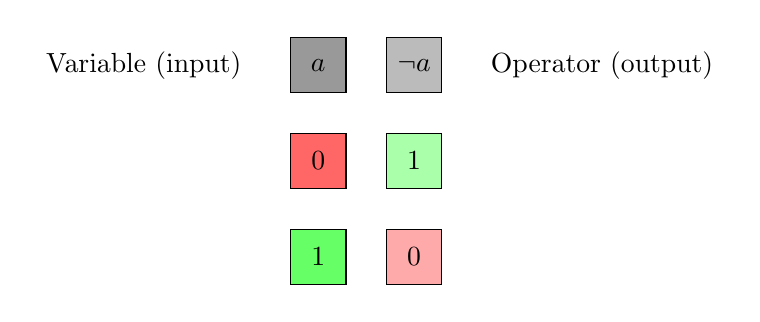
\begin{tikzpicture}[ampersand replacement=\&]
      \matrix[row sep = 5mm, column sep = 5mm] at (0, 0) {  
        \onslide<2->{ \node[label]{Variable (input)}; }
        \& \node[var]{$a$}; 
        \& \node[oper]{$\neg a$};
        \& \onslide<2->{ \node[label]{Operator (output)}; } \\
        
        \& \onslide<3->{ \node[if]{0}; }
        \&  \onslide<4->{ \node[ot]{1}; } \\ 
        
        \&  \onslide<5->{ \node[it]{1}; }
        \&  \onslide<6->{ \node[of]{0}; } \\
      };
    \end{tikzpicture}

    \medskip
    
    \onslide<7-11>{ This is called \textit{negation}. }
    
  \end{center}


  
\end{frame}



\end{document}
